\section{Security and Privacy Analysis}
\label{sec:analysis}

%We define three adversarial scenarios under the threat model in Section \ref{subsec:threatmodel}, develop a Dolev-Yao style model \cite{BrowserID} to formalize the SSO login flow in \usso, and then integrate its conclusions to formally prove the security and privacy guarantees provided by \usso.

We prove the security and privacy guarantees provided by \usso.
It is worth noting that these guarantees are proved against different adversaries.


\subsection{Adversarial Scenarios}

Based on our design goals (i.e., the desired security and privacy guarantees) and the potential adversaries discussed in Section \ref{subsec:threatmodel}, we consider three adversarial scenarios as below.

\noindent\textbf{Adversaries against security.} Malicious users could collude with each other and even with malicious RPs \cite{FettKS14,BrowserID,SPRESSO}, attempting to (\emph{a}) impersonate an honest user to log into an honest RP or (\emph{b}) entice an honest user to log into an honest RP under another user's account.

\noindent\textbf{Adversaries against IdP untraceability.}
The honest-but-curious IdP tries to infer the identities of the RPs that an honest user requests to visit. %or link multiple logins to any RP initiated by a user.

\noindent\textbf{Adversaries against RP unlinkability.}
Malicious RPs could collude with each other and even malicious users, attempting to link logins across these RPs initiated by honest users. 

%\oldc


% \subsection{The Dolev-Yao Style Model for \usso}
% \label{dy-model}

% We develop a Dolev-Yao style model \cite{BrowserID, SPRESSO, FettKS16, FettKS17} for \usso, referred to as the \emph{\dyu\ model}, to formalize the login flow of \usso.
% % Dolev-Yao style models abstract cryptographic concepts into an algebra of symbolic messages to discover structural flaws using simple formal logic. % which has been used in the formal analysis of SSO protocols such as OAuth 2.0 \cite{FettKS16} and OIDC \cite{FettKS17}.
% The model abstracts the entities in a web system, such as web servers and browsers, as atomic processes, %which communicate with each other through events. % such as HTTPS requests and responses.
% and defines scripting processes to formulate client-side scripts.
% %The script is dependently invoked by the browser to process the server-defined logic.%such as verifying $Certificate_{RP}$. %postmessage events; %atomic process <-> scripting process, communication. %Other events change self-trigger.
% The atomic processes of \usso\ include an IdP process, a finite set of web servers for honest RPs, a finite set of honest browsers, and a finite set of attacker processes that model malicious RPs and malicious users.
% A browser may invoke an honest IdP script and multiple RP scripts that could be honest or malicious.
% The processes communicate with each other through events such as HTTPS requests and responses,
% %Although the scripts coexist in the same browser, they are strictly separated.
% except that the scripting processes communicate with each other through \verb+postMessage+ which are modeled as transmitted-to-itself events of a browser process.
% %To clearly indicate the action of postMessage communication, we define it as the transmitting-to-itself event of the browser (which is not defined in SPRESSO).


% Applying the \dyu\ model, we trace the lifecycle of an identity token from its generation at the IdP to its acceptance at an RP, locate the places where $PID_U$, $PID_{RP}$, and other elements related to the identity token such as $t$ and $u$ are processed, and locate the places where $PK$ is transmitted and used in the IdP script.
% We confirm the following conclusions in the \dyu\ model:
% (\emph{a}) an identity token binding pseudo-identities of honest entities, cannot be leaked to any malicious process;
% (\emph{b}) pseudo-identities and other elements in verified identity tokens cannot be manipulated by any malicious process;
% (\emph{c}) the IdP's public key set in the IdP script cannot be replaced or tampered with by any malicious process, within an honest browser;
% (\emph{d}) the IdP receives nothing about $t$ shared between two honest processes;
% (\emph{e}) $r$ is not leaked to any malicious process as it never leaves the IdP;
% and (\emph{f}) the RPs cannot receive anything about $u$ shared between two honest processes.


\subsection{Security}
\label{analysis-security}

%could collude with each other and even with malicious RPs, attempting to (\emph{a}) impersonate an honest user to log into an honest RP or (\emph{b}) entice an honest user to log into an honest RP under a malicious user's account.

In secure SSO systems, an identity token $TK$ which is requested by a user to visit an RP,
    enables only this user to log into only the honest target RP exactly as her account at this RP.
When confidentiality and integrity of $TK$ are ensured by secure communications and digital signatures in \usso, we summarize the following necessary and sufficient conditions of secure SSO services \cite{FettKS14,BrowserID,SPRESSO}:

\noindent \textbf{RP Designation.} $TK$ designates the target RP,
    and only the designated (honest) RP derives a meaningful account which responds to some registered user after accepting $TK$.
That is, at other honest RPs, no meaningful account will be derived.

\noindent \textbf{User Identification.} At the designated RP, $TK$ identifies only the user who requests this token from the IdP. That is, the designated honest RP will derive only the account exactly corresponding to the identified user.



%------- old Theorem 5 ---------
\begin{comment}
\begin{thm}
\textsc{(Security)} \emph{\usso\ provides secure authentication services.}
\end{thm}

\noindent\textbf{\textsc{Proof.}}
According to the formal analysis on SSO security \cite{SPRESSO, FettKS14},
    an SSO system satisfying the following two requirements provides \emph{secure} authentication services in the first adversarial scenario: (\emph{a}) an adversary never obtains a valid identity token issued for an honest user and presents it to an honest RP, and (\emph{b}) an honest user never presents a valid identity token that is not issued for herself to an honest RP.

Following the login flow of \usso, because the integrity and confidentiality of identity tokens are satisfied in Theorems \ref{thm-integrity} and \ref{thm-confidentiality},
 no adversary could obtain a valid identity token that is issued to an honest user for accessing an honest RP. %and accepted by an honest RP.
Meanwhile, if an adversary presents an identity token to an honest RP, which may be issued to the adversary for accessing another RP or to an honest user for accessing a colluding RP, RP designation and user identification, proved in Theorems \ref{thm-rp-designation} and \ref{thm-user-id}, ensure that the honest RP does not derive an honest user's account from this identity token.
%Meanwhile, $PID_U$ can only be calculated by the IdP and the user, since no one else knows or could intercept $u$ according to the DYU model. \oldc

According to the login flow and the \dyu\ model, an honest user always obtains identity tokens issued to herself, because $PID_U$ is calculated based on her identity. 
%% which is protected against adversaries. 这一句,对于security没有用,protecting u是用于privacy。
The confidentiality and integrity of identity tokens ensure that an honest user never presents any token issued for someone else to an honest RP. Finally, with user identification,\footnote{\newc RP designation is a precondition of user identification in \usso, but this is not always necessary for other SSO systems.} her identity tokens are always associated with her account at the target RP.
%According to the conclusions of the DYU model, $PID_U$ is calculated based on the user when the IdP issues an identity token for an authenticated user.
%Moreover, because the confidentiality and integrity of identity tokens are satisfied, an honest user never presents a valid token that is issued to other users.
%When the user identification is satisfied, this token always derives this honest user's account.
%So, an honest user never presents an identity token that is accepted by an honest RP to derive another user’s account at this RP.

Thus, \usso\ is a secure SSO system.
\hfill $\square$

%Finally, according to Theorems 1, 2, 3, 4, and 5, UPPRESSO is secure.

\end{comment}


%We prove that identity tokens in \usso\ and the enclosed pseudo-identities satisfy four properties, namely, \emph{RP designation}, \emph{user identification}, \emph{token confidentiality}, and \emph{token integrity}, which together ensure the security of \usso\ in the first adversarial scenario.

Let's assume totally $s$ users and $p$ RPs in \usso,
    whose identities are denoted as $\mathbf{u} = \{u_{i; 1 \leq i \leq s}\}$ and $\mathbb{ID}_{RP} = \{[r_{j;1 \leq j \leq p}]G\}$, respectively.
Therefore, there are accounts $Acct_{i,j}=[u_i]ID_{RP_j} = [u_i r_j]G$ $(1 \leq i \leq s)$ automatically registered at each RP.
Because $[r_j]G$ is also a generator on $\mathbb{E}$ of order $n$,
    at each RP $Acct_{i,j}=[u_i r_j]G$ is \emph{unique} for $u_i$ is unique in $\mathbb{Z}_n$.
Accounts are publicly-known, but $u_{i}$ and $r_{j}$ are unknown to adversaries.

We prove that, in \usso\ 
an identity token binding $PID_{RP} = [t]ID_{RP}$ and $PID_U = [u]PID_{RP}$, which is requested by an authenticated user with $ID_U =u$ to visit an RP with $ID_{RP}$,
    satisfies RP designation and user identification.

\vspace{-1.2mm}
\begin{thm}[RP Designation]
\emph{Given $u \in \mathbf{u}$ and $ID_{RP} \in \mathbb{ID}_{RP}$,
from $TK$ binding $PID_{RP}=[t]ID_{RP}$ and $PID_U = [u]PID_{RP}$,
    any honest RP with ${ID_{RP'} \neq ID_{RP}}$ cannot derive $Acct = [u']ID_{RP'}$ where $u' \in \mathbf{u}$ and $ID_{RP'} \in \mathbb{ID}_{RP}$.}\label{thm-rp-designation}
\end{thm}
\vspace{-1.2mm}

\noindent\textbf{\textsc{Proof.}} 
A malicious user colluding with malicious RPs,
    might forward $TK$ to some honest RP other than the designated RP,
        even with a manipulated trapdoor $t'$.
Then, this deceived RP derives $Acct = [t'^{-1}]PID_U = [t'^{-1}utr]G$.

Next, we prove that, when $u_{i; 1\leq i \leq s}$ and $r_{j; 1\leq j \leq p}$ are unknown,
    for any $[r']G \neq [r]G$ where $[r']G \in \mathbb{ID}_{RP}$,
    the adversaries cannot find $t$ and $t'$ satisfying $[t'^{-1}utr]G = [u'r']G$ where $u' \in \mathbf{u}$.
This attack can be described as an account-collision game $\mathcal{G}_A$ between an adversary and a challenger:
 the adversary receives from the challenger a set of RP identities $\mathbb{ID}_{RP}$,
  $ID_{RP_{a}}$ and a set of accounts $\{Acct_{i,j}= [u_ir_j]G\}$,
 and then outputs $(i_1, i_2, b, t, t')$ where $b \neq a$ and $b \in [1,p]$.
If $[t'^{-1}t]Acct_{i_1,r_a} = [t'^{-1}u_{i_1}tr_{a}]G = [u_{i_2}r_{b}]G = Acct_{i_2,r_b}$, which occurs with a probability ${\rm Pr}_s$, the adversary succeeds.

\begin{figure}[tb]
  \centering
  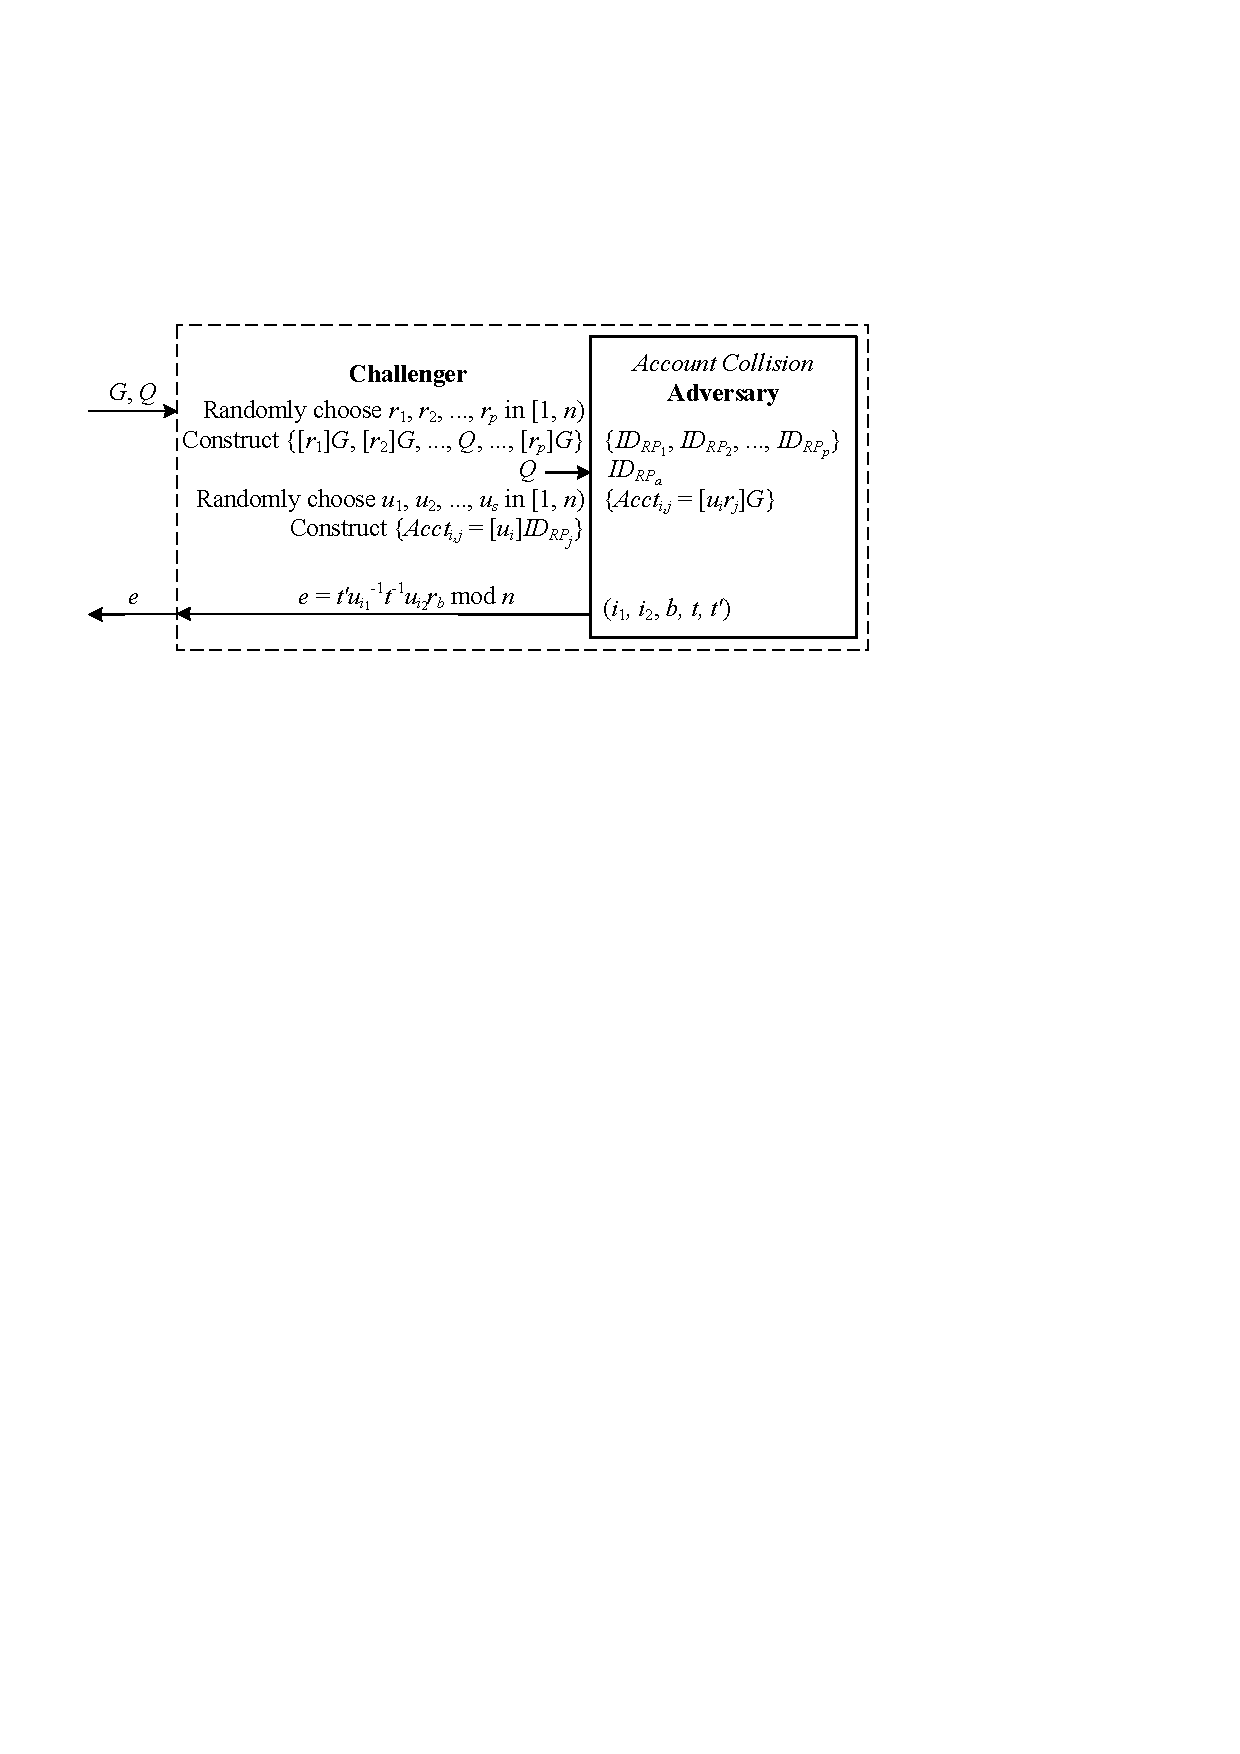
\includegraphics[width=0.96\linewidth]{fig/ecdlp_algorithm2.pdf}
  \caption{The PPT algorithm $\mathcal{D}^*_A$ constructed based on the account-collision game to solve the ECDLP.}
  \label{fig:collision_account}
\end{figure}

As depicted in Figure \ref{fig:collision_account}, we design a probabilistic polynomial time (PPT) algorithm $\mathcal{D}^*_A$ based on $\mathcal{G}_A$, to solve the ECDLP: find a number $x \in \mathbb{Z}_n$ satisfying $Q = [x]G$, where $Q$ is a point on $\mathbb{E}$ and $G$ is a generator on $\mathbb{E}$ of order $n$.

The algorithm $\mathcal{D}^*_A$ works as below.
The input of $\mathcal{D}^*_A$ is in the form of ($G, Q$). On receiving an input, the challenger firstly chooses $r_1, \cdots, r_p$  random in $\mathbb{Z}_n$ to calculate $\{[r_{j;1\leq j \leq p}]G\}$,
 randomly chooses $a \in [1,p]$ to replace $[r_{a}]G$ with $Q$,
 and constructs $\mathbb{ID}_{RP} = \{[r_1]G, \cdots, Q, [r_{a+1}], \cdots, [r_{p}]G\}$.
The challenger also chooses $u_1, \cdots, u_s$ random in $\mathbb{Z}_n$ to calculate $\{Acct_{i,j}= [u_{i;1\leq i \leq s}]ID_{RP_{j;1 \leq j \leq p}}\}$.
Then, it sends $\mathbb{ID}_{RP}$, $Q$ and $\{Acct_{i,j}\}$ to the adversary, which returns the result $(i_1, i_2, b, t, t')$.
 Finally, the challenger calculates $e = t'u_{i_1}^{-1}t^{-1}u_{i_2}r_{b} \bmod n$, and sets $e$ as the output of $\mathcal{D}^*_A$.

If $[t'^{-1}u_{i_1}t]Q = [u_{i_2}r_{b}]G$ and the adversary succeeds in $\mathcal{G}_A$, $\mathcal{D}^*_A$ outputs $e =x$
 because $Q = [t'u_{i_1}^{-1}t^{-1}u_{i_2}r_{b}]G$.
If the adversary would have advantages  in $\mathcal{G}_A$ and ${\rm Pr}_s$ is non-negligible regardless of the security parameter $\lambda$,
    we would find that ${\rm Pr}\{\mathcal{D}^*_A(G, [x]G)=x\}= {\rm Pr}_s$ also becomes non-negligible even when $\lambda$ is sufficiently large.
This violates the ECDLP assumption.
Therefore, the probability that the adversary succeeds in $\mathcal{G}_A$ is negligible,
    and RP designation is ensured.
\hfill $\square$
\vspace{.75mm}

Because $TK$ works only at the ``implicitly'' designated RP and
    no meaningful user will be derived at any other RPs, % when $u_i$ and $r_j$ are kept unknown to adversaries,
 in Step 4.2 an RP does not check whether $PID_{RP}$ in the received token equals to $[t]ID_{RP}$ or not.


\vspace{-1.2mm}
\begin{thm}[User Identification] \emph{Given $u \in \mathbf{u}$ and $ID_{RP} \in \mathbb{ID}_{RP}$,
from $TK$ binding $PID_{RP}=[t]ID_{RP}$ and $PID_U = [u]PID_{RP}$,
 the meaningful account derived at the honest RP with $ID_{RP}$ 
 is only $Acct = [u]ID_{RP}$.}\label{thm-user-id}
\end{thm}
\vspace{-1.2mm}

\noindent\textbf{\textsc{Proof.}}
Firstly, on receiving $t$,
the RP designated by $TK$ calculates $Acct = [t^{-1}]PID_{U} =[t^{-1}ut]ID_{RP} = [u]ID_{RP}$,
    exactly corresponding to the authenticated user.
% which is a \emph{permanent} identifier determined by $ID_U$ and $ID_{RP}$.
%$ID_{RP} = [r]G$ is also a generator on $\mathbb{E}$ of order $n$, as $\mathbb{E}$ is a finite cyclic group. Therefore, given a user with $ID_U$, $Acct$ is a \emph{unique} point on $\mathbb{E}$ for any $u \in [1, n)$, and it is \emph{uniquely} associated with $ID_U=u$. 
%We first prove that $PID_{U}$ \emph{uniquely} identifies one account at the designated RP and one user in the system. 
%This proves that $PID_U$ in $TK$ identifies an account $Acct$ at the designated RP, which is uniquely mapped to a user with $ID_U$ in the system.

We consider $TK$ replayed by malicious users to the target RP, but with a manipulated trapdoor $t' \neq t$.
The designated RP will derive another account $[t'^{-1}]PID_U = [t'^{-1}ut]ID_{RP}$.
Because $G$ is a generator on $\mathbb{E}$ of order $n$, $ID_{RP}$ and $[ut]ID_{RP}$ are also generators on $\mathbb{E}$.
Therefore, when $u_{i; 1\leq i \leq s}$ are unknown, the probability that $[t'^{-1}ut]ID_{RP}$ happens to be another meaningful account $[u_i]ID_{RP}$ at this RP is $\frac{s-1}{n}$,
because $u_i$ is randomly selected in $\mathbb{Z}_n$ by the IdP.

This probability becomes negligible, when $n$ is sufficiently large.
As a result, $[t'^{-1}]PID_U$ $(t' \neq t)$ does not result in any meaningful account at the designated RP. 
%Secondly, the attacker presents $TK$ to another RP with $ID_{RP'} = [r']G \neq [r]G$. This RP will calculate the account as $Acct' = [\tilde{t}^{-1}]PID_{U} = [\tilde{t}^{-1}utrr'^{-1}][r']G = [\tilde{t}^{-1}utrr'^{-1}]ID_{RP'}$. The probability that $\tilde{t}^{-1}utrr'^{-1}$ happens to be the identity of another registered user at this RP is also negligible, when $n$ is sufficiently large. 
%it identifies no account mapped to a user, at any RP not designated by $PID_{RP}$.
\hfill $\square$



%---- remove Theorem 4 and 5 and move the proofs to Appendix
% \begin{thm}
% \textsc{(Token Integrity)} \emph{An identity token issued by the IdP cannot be forged or manipulated.}
% \label{thm-integrity}
% \end{thm}

% \noindent\textbf{\textsc{Proof.}} Identity tokens are generated and signed by the honest IdP using its private key, which is sufficiently protected at the IdP against adversaries.
% %Meanwhile, the IdP's public key $PK$ is sent from the IdP to the RPs.
% %and $PK$ which are pre-installed by an RP cannot be manipulated by adversaries.
% With the pre-installed public key, an RP verifies the identity tokens it receives and rejects any forged or manipulated identity tokens. Finally, according to the conclusions of the DYU model, the elements in a verified token cannot be manipulated by malicious entities.
% \hfill $\square$


% \begin{thm}
% \textsc{(Token Confidentiality)} \emph{An identity token is accessible only to its designated RP, besides the requesting user and the IdP.}
% \label{thm-confidentiality}
% \end{thm}

% \noindent\textbf{\textsc{Proof.}}
% An identity token is generated by the IdP and then sent to the requesting user (i.e., its IdP script).
% The IdP script verifies if $ID_{RP}$ specified in a verified RP certificate is designated by $PID_{RP}$ in the identity token and forwards the token to the correct RP script, which is downloaded from the origin of $Enpt_{RP}$ specified also in the RP certificate. %Because the IdP script calculates $PID_{RP} =[t]ID_{RP}$ based on $ID_{RP}$ in this verified RP certificate, this RP is designated in the identity token and will receive the token from the RP script.
% As all the communications between the IdP, RPs, and users are protected by HTTPS and two scripts communicate with each other through restricted \verb+postMessage+ HTML5 channels, according to the conclusions of the \dyu\ model, the identity tokens cannot be leaked to any other entities. \hfill $\square$

%--- End of Theorem 4 and 5

\subsection{Privacy against IdP-based Login Tracing}
\label{subsec:IdP-privacy}

In \usso\ the \emph{curious} IdP would attempt to infer the RP's identities visited by a user. Since the IdP is considered \emph{honest}, it only collects information from the identity-token requests, % to infer the visited RPs' identities,
 but does not deviate from the protocol or collude with others.

The IdP does not obtain any information related to the target RP in each login (e.g., $ID_{RP}$, $Enpt_{RP}$ or $Cert_{RP}$), except its \emph{ephemeral} pseudo-identity $PID_{RP}$.
We prove in Theorem \ref{thm-idp-untraceability} that, from these $PID_{RP}$s in the identity-token requests,
 the IdP cannot (\emph{a}) associate multiple logins to the same RP, or (\emph{b}) distinguish a login to one RP from other logins to another RP, because to the IdP $PID_{RP}$ is \emph{indistinguishable} from a random variables on $\mathbb{E}$. So \usso\ prevents the honest-but-curious IdP from tracing a user's login activities.

\vspace{-1.2mm}
\begin{thm}[IdP Untraceability]
\emph{In \usso, the IdP cannot distinguish $PID_{RP} = [t]ID_{RP}$ from a random variable on $\mathbb{E}$, where $t$ is random in $\mathbb{Z}_n$ and kept unknown to the IdP.}\label{thm-idp-untraceability}
\end{thm}
\vspace{-1.2mm}

\noindent\textbf{\textsc{Proof.}}
$\mathbb{E}$ is a finite cyclic group, and the number of points on $\mathbb{E}$ is $n$.
Because $G$ is a generator of order $n$, $ID_{RP} = [r]G$ is also a generator on $\mathbb{E}$ of order $n$. %According to the formal model in Appendix \ref{appendix-model}, 
When $t$ is randomly chosen in $\mathbb{Z}_n$ and unknown to the IdP, $PID_{RP} = [t]ID_{RP}$ is \emph{indistinguishable} from a point that is randomly chosen on $\mathbb{E}$ \cite{oprf-proved,voprf-proved}. \hfill $\square$
\vspace{.75mm}

This property of obliviousnes actually has been proved in OPRFs \cite{oprf-proved,voprf-proved}, where the OPRF server works similarly to the IdP and learns \emph{nothing} about a client's inputs or outputs of the evaluated pseudo-random function.

\subsection{Privacy against RP-based Identity Linkage}
\label{subsec:RP-privacy}

Malicious RPs,
which could collude with some malicious users,
aim to infer the identities of honest users
    or link an honest user's accounts across these RPs.


In each login, an RP obtains \emph{only} a random number $t$ and an identity token enclosing $PID_{RP}$ and $PID_U$. From the token, it learns only an ephemeral pseudo-identifier $PID_{U} = [{ID_U}]{PID_{RP}}$ of the user, from which it derives a permanent pseudo-identifier $Acct = [ID_U]ID_{RP}$. However, it cannot directly calculate $ID_U$ from $PID_{U}$ or $Acct$ due to the ECDLP.
%Next, we show that, with Property {\bf C1}, \usso\ prevents malicious RP(s) from reading or altering the identity token request sent by the IdP script that runs in an honest browser to the IdP. Therefore, the RP obtains no knowledge about the user identity $ID_U$. Meanwhile, following the formal model in Appendix \ref{appendix-model}, we see that the RP script running in an honest browser is always honest, no matter if the RP would be corrupted at a later time or not. A script download from a malicious RP would not be installed by an honest user. 
Next, we prove in Theorem \ref{thm-rp-unlinkability} that, even if malicious RPs collude with each other and some malicious users by sharing $PID_U$s and other information observed in all the logins, they still cannot link any login from an honest user to any other logins from any honest users to other colluding RPs.

%\usso\ prevents the privacy threats of \emph{RP-based identity linkage} against \emph{malicious RPs which collude with malicious users}, attempting to link the logins initiated by an honest user but visiting different colluding RPs. 
%The IdP does not collude with the adversaries in this scenario.

%Therefore, the colluding adversaries share all logins visiting malicious RPs, and attempt to leverage the logins initiated by malicious users to link the other logins by honest users.


With the trapdoor $t$, $PID_{RP}$ and $PID_U$ can be easily transformed into $ID_{RP}$ and $Acct$, respectively, and vice versa.
So we denote all the information that an RP learns in a login as a tuple $L$, where $L =(ID_{RP}, t, Acct)=(ID_{RP}, t, [ID_{U}]ID_{RP})=([r]G, t, [ur]G)$.


%Hence, an $RP_j$ with $w$ logins knows $\{L_{1,j},...,L_{w,j}\}$.

When $c$ malicious RPs collude with each other, they create a shared view of all their logins, denoted as $\mathbb{L}$.
%some of which are initiated by honest users and denoted as $\mathbb{L}^h$, and the others by $v$ malicious users  are $\mathbb{L}^m = \mathbb{L} \setminus \mathbb{L}^h$.
When they collude further with $v$ malicious users, the logins initiated by these malicious users are picked out of $\mathbb{L}$ and linked together as
$\mathfrak{L}^m=\left \{ \begin{matrix}
L^m_{1,1},&L^m_{1,2},&\cdots,&L^m_{1,c}\\
L^m_{2,1},& L^m_{2,2},&\cdots,&L^m_{2,c}\\
\cdots,&\cdots,&L^m_{i,j},&\cdots\\
L^m_{v,1},&L^m_{v,2},&\cdots,&L^m_{v,c}
\end{matrix}\right\}$,
where $L^m_{i, j}=([r_j]G, t_{i,j}, [u_ir_j]G) \in \mathbb{L}$ for $1 \le i \le v$ and $1 \le j \le c$. Any login in $\mathbb{L}$ but not linked in $\mathfrak{L}^m$ is initiated by an honest user to one of the $c$ malicious RPs.

\begin{figure}[tb]
  \centering
  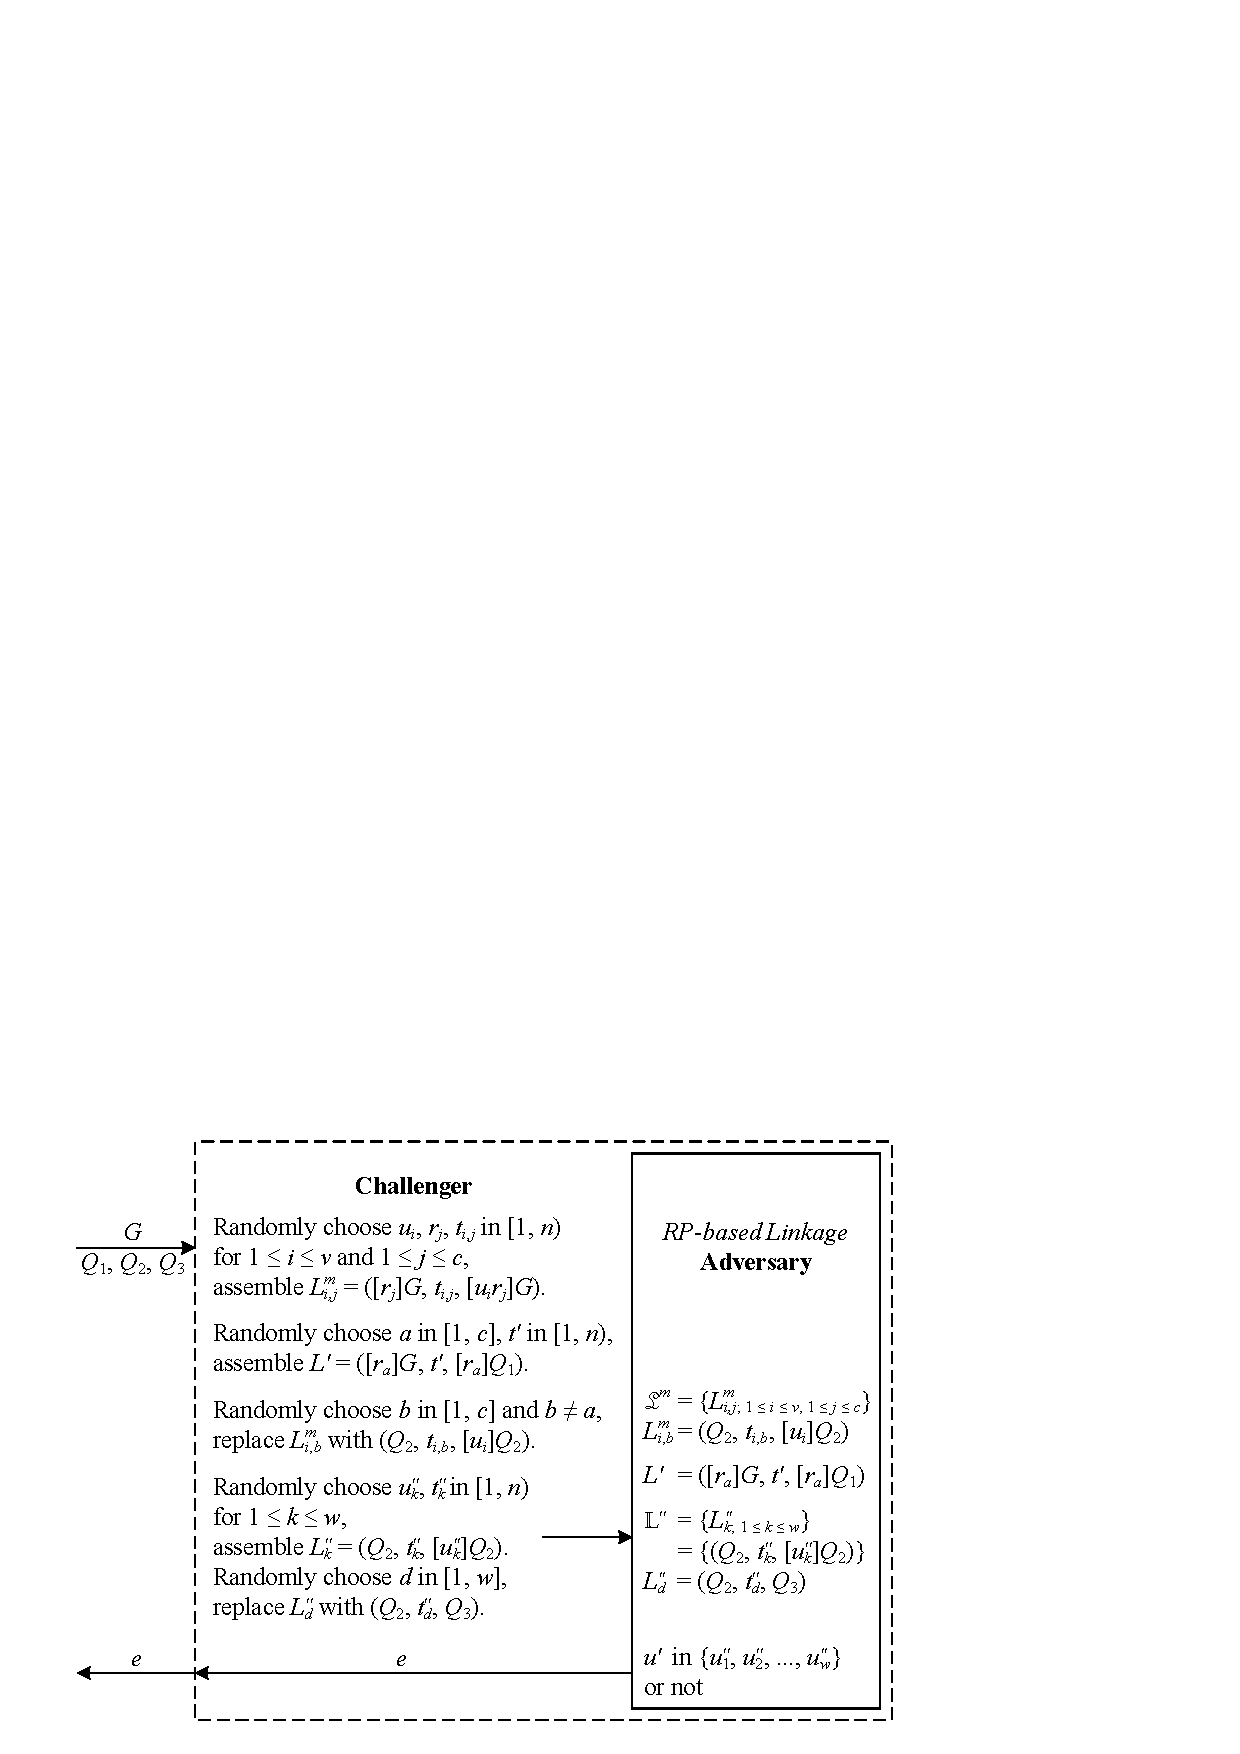
\includegraphics[width=1.0\linewidth]{fig/rp-linkage-game.pdf}
  \caption{The PPT algorithm $\mathcal{D}^*_R$ constructed based on the RP-based linkage game to solve the ECDDH problem.}
  \label{fig:dalgorithm}
\end{figure}


%\vspace{-1.2mm}
\begin{thm}[RP Unlinkability]
\emph{In \usso, given $\mathbb{L}$ and $\mathfrak{L}^m$, $c$ malicious RPs and $v$ malicious users cannot link any login from an honest user to some malicious RP to any subset of logins from honest users to any other malicious RPs.}\label{thm-rp-unlinkability}
\end{thm}
\vspace{-1.2mm}

\noindent\textbf{\textsc{Proof.}} From the logins in $\mathbb{L}$,
 we randomly choose one login $L' \neq L^m_{i,j}$ $(1 \le i \le v, 1 \le j \le c)$,
 which is initiated by an (unknown) honest user with $ID_{U'}=u'$ to a malicious $RP_{a}$ where $a \in [1,c]$.
Then, we randomly choose another malicious $RP_{b}$, where $b \in [1,c]$ and $b \neq a$.
Consider any subset $\mathbb{L}'' \subset \mathbb{L}$ of $w$ logins visiting $RP_{b}$ by unknown honest users,
 we denote the identities of the honest users who initiate these logins as $\mathbf{u}^w=\{{u''_1}, {u''_2}, \cdots, {u''_w}\}$.
Next, we prove that the colluding adversaries cannot decide if $u'$ is in $\mathbf{u}^w$ or randomly selected from the universal user set.
This indicates that the colluding adversaries cannot link $L'$ to another login (or a subset of logins) visiting $RP_{b}$.


We define an RP-based linkage game $\mathcal{G}_R$ between an adversary and a challenger, which describes this login linkage threat: the adversary receives $\mathfrak{L}^m$, $L'$, and $\mathbb{L}''$ from the challenger and outputs $e$, where (\emph{a}) $e = 1$ if it decides $u'$ is in $\mathbf{u}^w$ %$\{{U''_1}, {U''_2}, \cdots, {U''_w}\}$
or (\emph{b}) $e=0$ if it believes $u'$ is randomly chosen from the universal user set.
Thus, the adversary succeeds in $\mathcal{G}_R$ with an advantage $\mathbf{Adv}$:
\begin{align*}
%&{\rm Pr}_1={\rm Pr}\{\mathcal{G}_r(\mathfrak{L}, L', \mathbb{L}'' | u' \in \{{u''_1}, {u''_2}, \cdots, {u''_w}\})=1\} \\
&{\rm Pr}_1={\rm Pr}(\mathcal{G}_R(\mathfrak{L}^m, L', \mathbb{L}'')=1 \;| \; u' \in \mathbf{u}^w)  \\
%&{\rm Pr}_2={\rm Pr}\{\mathcal{G}_r(\mathfrak{L}, L', \mathbb{L}'' | u' \in \mathbb{Z}_n)=1\}\\
&{\rm Pr}_2={\rm Pr}(\mathcal{G}_R(\mathfrak{L}^m, L', \mathbb{L}'')=1 \; | \; u' \in \mathbb{Z}_n)\\
&{\mathbf{Adv}}=|{\rm Pr}_1-{\rm Pr}_2|
\end{align*}

As depicted in Figure \ref{fig:dalgorithm}, we then design a PPT algorithm $\mathcal{D}^*_R$ based on $\mathcal{G}_R$ to solve the elliptic curve decisional Diffie-Hellman (ECDDH) problem: given $(G, [x]G$, $[y]G$, $[z]G)$, decide whether $z$ is equal to $xy$ or randomly chosen in $\mathbb{Z}_n$, where $G$ is a point on an elliptic curve $\mathbb{E}$ of order $n$, and $x$ and $y$ are integers randomly and independently chosen in $\mathbb{Z}_n$.


The algorithm $\mathcal{D}^*_R$ works as below. (1) Upon receiving an input $(G, Q_1=[x]G, Q_2=[y]G, Q_3=[z]G)$, %of $\mathcal{D}^*_r$
the challenger
chooses random numbers in $\mathbb{Z}_n$ to construct $\{u_i\}$, $\{r_j\}$, and $\{t_{i, j}\}$ for $1 \le i \le v$ and $1 \le j \le c$, with which it assembles $L^m_{i, j}=([r_j]G, t_{i,j}, [u_ir_j]G)$.
In this process, it ensures $[r_{j}]G \neq Q_2$ so that $r_j \neq y$.  % 这个应该反过来讲;因为y是离散对数。
(2) It randomly chooses $a \in [1, c]$ and $t' \in \mathbb{Z}_n$, to assemble $L' = ([r_{a}]G, t', [r_{a}]Q_1) = ([r_{a}]G, t', [xr_{a}]G)$.
(3)
% Here, $L'$ represents the knowledge of the login visiting $RP_{j'}$ by a user with $ID_U = x$.
Next, the challenger randomly chooses $b \in [1, c]$ and $b \neq a$, and replaces $ID_{RP_b}$ with $Q_2 = [y]G$.
Hence, for $1 \le i \le v$, the challenger replaces $L^m_{i, b}=([r_b]G, t_{i,b}, [u_ir_b]G)$ with $(Q_2, t_{i,b}, [u_i]Q_2) = ([y]G, t_{i,b}, [u_iy]G)$, and then constructs $\mathfrak{L}^m$.
(4) The challenger chooses random numbers in $\mathbb{Z}_n$ to construct $\{u''_k\}$ and $\{t''_k\}$ for $1 \leq k \leq w$,
 with which it assembles $\mathbb{L}'' = \{L''_{k; 1\leq k \leq w}\} = \{(Q_2, t''_k, [u''_k]Q_2)\} = \{([y]G, t''_k, [u''_ky]G)\}$.
In this process, it ensures that $[u''_k]G \neq Q_1$ (i.e., $u''_k \neq x$) and $u''_k \neq u_i$,
 for $1 \le i \le v$ and $1 \le k \le w$.
Finally, it randomly chooses $d \in [1, w]$ and replaces $L''_{d}$ with $(Q_2, t''_d, Q_3) = ([y]G, t''_d, [z]G)$.
 Thus, $\mathbb{L}'' = \{L''_{k;1\leq k \leq w}\}$ represents the logins initiated by $w$ honest users, i.e., $\mathbf{u}^w=\{u''_1, u''_2, \cdots, u''_{d-1}, z/y, u''_{d+1}, \cdots, u''_w\}$.
 (5) When the adversary of $\mathcal{G}_R$ receives $\mathfrak{L}^m$, $L'$, and $\mathbb{L}''$ from the challenger, it returns $e$ which is also the output of $\mathcal{D}^*_R$.

According to the above construction, % of $\mathfrak{L}$, $L'$ and $\mathbb{L}''$,
$x$ is embedded as $ID_{U'}$ in the login $L'$ visiting the RP with $ID_{RP_{a}} = [r_{a}]G$,
and $z/y$ is embedded as $ID_{U''_d}$ in $\mathbb{L}''$ visiting the RP with $ID_{RP_{b}}=[y]G$,
together with $\{u''_1, \cdots, u''_{d-1}, u''_{d+1}, \cdots, u''_w\}$.
Meanwhile, $[r_{a}]G$ and $[y]G$ are two malicious RPs' identities in $\mathfrak{L}^m$.
Because $x \neq u''_{k; 1\leq k \leq w, k \neq d}$ and then $x$ is not in $\{u''_1, \cdots, u''_{d-1}, u''_{d+1}, \cdots, u''_w\}$, the adversary outputs $s=1$ and succeeds in the game \emph{only if} $x = z/y$.
% 这里不是if and only if. "if, 就变成了the adversary必胜了;并不是,而是“有显著的概率”"
% 当“the adversary outputs s=1 且 succeeds in the game”,=> "x = z/y"
% 但是,"x = z/y"  => 不能推导得到“the adversary outputs s=1 且 succeeds in the game”。因为adversary有时候fail、不总是succeed
 Therefore, using $\mathcal{D}^*_R$ to solve the ECDDH problem, we have an advantage $\mathbf{Adv}^*=|{\rm Pr}^*_1 - {\rm Pr}^*_2|$, where
\begin{align*}
&{\rm Pr}^*_1 =  {\rm Pr}(\mathcal{D}^*_R(G, [x]G, [y]G, [xy]G)=1) \\
=&{\rm Pr}(\mathcal{G}_R(\mathfrak{L}^m, L', \mathbb{L}'')=1 \; | \; u' \in \mathbf{u}^w) = {\rm Pr}_1 \\
&{\rm Pr}^*_2= {\rm Pr}(\mathcal{D}^*_R(G, [x]G, [y]G, [z]G)=1) \\
=&{\rm Pr}(\mathcal{G}_R(\mathfrak{L}^m, L', \mathbb{L}'')=1 \; | \; u' \in \mathbb{Z}_n) = {\rm Pr}_2 \\
&\mathbf{Adv}^*=|{\rm Pr}^*_1-{\rm Pr}^*_2|=|{\rm Pr}_1-{\rm Pr}_2|={\mathbf{Adv}}
\end{align*}

If in $\mathcal{G}_R$ the adversary has a non-negligible advantage, then $\mathbf{Adv}^*={\mathbf{Adv}}$ is also non-negligible regardless of the security parameter $\lambda$. This violates the ECDDH assumption.
 Therefore, the adversary has no advantage in $\mathcal{G}_R$ and cannot decide whether $L'$ is initiated by some user with an identity in $\mathbf{u}^w$ or by a user in the universal user set.
Because $RP_b$ is any malicious RP, this proof can be easily extended from $RP_b$ to more colluding malicious RPs.
\hfill $\square$


